%==================================
%              Decay 
%==================================
\section{\review{Accounting for Decay}}
\label{section:decapoles:decay}

FiDeL, the field model used in operation, aims at correcting the field errors at various energies.
Measured field errors but also decay estimates with respect to time are used when computing
corrections.

Magnetic decay in superconducting magnets stems from field changes in the strands caused by current
redistribution in the superconducting cables. Decay has been shown to be strongly dependent on the
magnet powering history~\cite{sammut_mathematical_2006,haverkamp_studies_1999}.
This happens for example when ramping down from an energy of 6.8 TeV to 0 and then going back to
injection energy at 450 GeV. Some components of the magnetic field will persist and gradually change
over time until they reach their final value.

While the sextupolar $b_3$ decay is accounted for during operations, a review of the FiDeL model
revealed that the decapolar component $b_5$ has not been similarly considered. To date, all beam
dynamics studies in the LHC have made use of the same set of magnetic measurement error tables, thus
neglecting any decapolar decay. It has though be found that during the LHC construction, magnetic
measurements were taken for a representative set of main dipoles, and decay measured.
%
The average $b_5$ field in the main dipoles at $t=0$, upon reaching the 450 GeV energy, is
approximately $1.145 \pm 0.5$, based on data from the magnetic reports utilized by FiDeL. For
reference, decay measurements of a selection of main dipoles (each dot), over time are illustrated
in \cref{fig:decapoles:decay:decay_b5}.
%
\Cref{table:decapoles:decay:decay_b5} shows the decay expected at injection energy after a typical
cycle of machine operation. From this table, it is clear that decay accounts for a large part of the
$b_5$ at injection. About $40\%$ of the compensated $b_5$ at injection in the main dipoles can
indeed be attributed to the decay.

\begin{figure}[!htb]
    \centering
    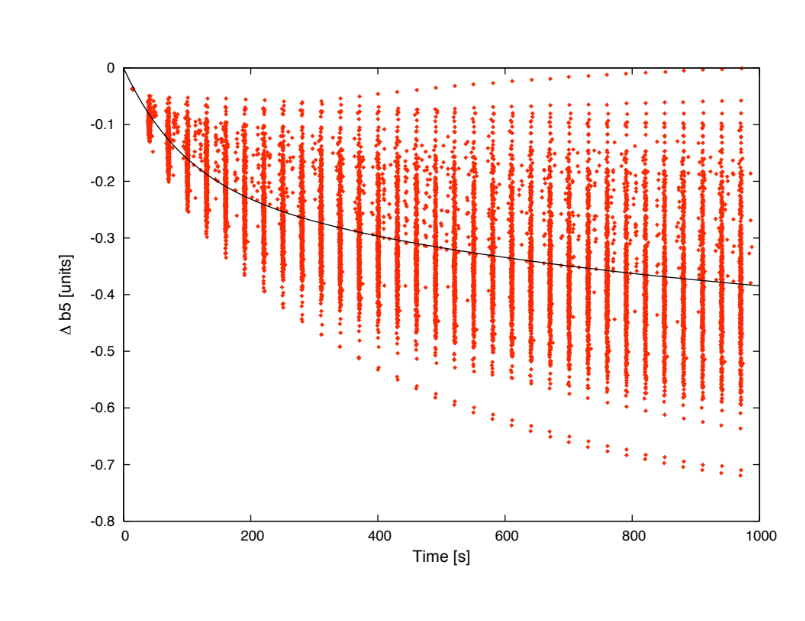
\includegraphics[width=0.7\textwidth]{./images/decay_b5_mb.pdf}
    \caption{Measured decay of the integrated decapolar field in LHC's main dipoles at injection
    energy. The fit is shown in black~\cite{deniau_magnetic_2009}.}
    \label{fig:decapoles:decay:decay_b5}
\end{figure}

\begin{table}[!htb]
    \centering
    \begin{tabular}{cl}
        \toprule
        Time [m] & $\Delta b_5$ \\
        \midrule
        $17$    & -0.38 \\ 
        $33$    & -0.44 \\
        $50$    & -0.46 \\
        $67$    & -0.47 \\
        $83$    & -0.47 \\
        $167$   & -0.47 \\
        \bottomrule
    \end{tabular}
    \caption{Decay of the $b_5$ component after injection for long time
    periods~\cite{deniau_magnetic_2009}.}
    \label{table:decapoles:decay:decay_b5}
\end{table}
 
Unfortunately, individual magnet measurements conducted more than 15 years ago could not be recovered. As
a result, the $b_5$ decay in the simulations is implemented as the average decay across all the
probed magnets. In the following simulations, each main dipole sees its $b_5$ component reduced by
$0.47$ units.


% ==== Chromaticity
\paragraph{Chromaticity}

It has been shown in the previous sections, and particularly in
\cref{table:decapoles:bare_chromaticity:virgin_dq3} that measurements and simulations were off
regarding the third order chromaticity $Q'''$.
New simulations have hence been conducted to evaluate the effect of this decay on chromaticity.
\Cref{table:decapoles:decay:simulation_chromaticity} compares simulations with and
without the decay of the $b_5$ component. The simulations use the 100 available error seeds to
calculate error bars.

\begin{table}[!htb]
    \centering
    \begin{tabular}{lll}
      \toprule
      Condition            & $Q'''_x [10^6]$ & $Q'''_y [10^6]$ \\
      \midrule
      No Decay             & $6.93 \pm 0.04$ & $-4.32 \pm 0.02$ \\
      $\Delta b_5 = -0.47$ & $4.05 \pm 0.04$ & $-2.54 \pm 0.02 $ \\
      \bottomrule
    \end{tabular}
    \caption{Comparison of $Q'''_x$ and $Q'''_y$ for Beam 1 with and without decay of the $b_5$
    component of the main dipoles at injection energy. Included fields errors range from normal and
    skew sextupoles ($n=3$) to icosapole ($n=10$).}
    \label{table:decapoles:decay:simulation_chromaticity}
  \end{table}

Implementing the decay of the $b_5$ component of the main dipoles in the simulations has
significantly reduced the discrepancy between beam-based measurement and the magnetic model.
%
Using the values from the bare chromaticity measurement and updating
\cref{table:decapoles:bare_chromaticity:virgin_dq3} with the newly obtain data provides a more
accurate description of the magnetic model, as shown in
\cref{table:decapoles:decay:virgin_dq3_recompare}.


\begin{table}[!htb]
    \centering
    \begin{tabular}{rrrr}
      \toprule
      Quantity     &  Measured $[10^6]$        &  Simulated $[10^{6}]$          &   \multicolumn{1}{c}{Ratio}     \\
      \midrule
        \multicolumn{1}{l}{Beam 1}    &                             &                                &             \\
                $Q'''_x$ &       $ 2.95 \pm 0.04$      & $ 4.05 \pm 0.04$               &  $0.73 \pm 0.01$  \\
                $Q'''_y$ &       $-1.82 \pm 0.04$      & $-2.54 \pm 0.02$               &  $0.72 \pm 0.02$  \\
      %\midrule
        \multicolumn{1}{l}{Beam 2}    &                             &                                &             \\
                $Q'''_x$ &       $ 3.06 \pm 0.07$      & $ 4.27 \pm 0.03$               &  $0.72 \pm 0.02$  \\
                $Q'''_y$ &       $-1.72 \pm 0.02$      & $-2.55 \pm 0.01$               &  $0.67 \pm 0.01$ \\
      \bottomrule
    \end{tabular}
    \caption{Measured and simulated third order chromaticity with octupole and decapole correctors
    turned off. The simulations include field errors from normal and skew sextupoles to icosapole
    ($n=3$ to $n=10$). The $b_5$ component of the main dipoles has been updated to include decay.}
    \label{table:decapoles:decay:virgin_dq3_recompare}
\end{table}




% ==== Chromatic Amplitude Detuning
\paragraph{Chromatic Amplitude Detuning}

Similar to chromaticity, new simulations have been conducted for chromatic amplitude detuning.
\Cref{table:decapoles:decay:chromatic_ampdet} gives an overview of the newly computed values and 
the related ratios relative to the measurements, while \cref{figure:decapoles:decay:two_terms} gives
a visual clue.
A small difference in agreement can be observed between the direct term $\partial^2 Q_y / (\partial
J_y \partial \delta)$ and the crossterm. This may arise from the implementation of decay, which only
considers the average $b_5$ across all dipoles and may not fully capture the individual variations.
Nevertheless, both terms now demonstrate a better agreement with the model, similar to the trend seen
with chromaticity.


\begin{table}[H]
  \centering
  \begin{tabular}{lrr}
  \toprule
   Type  & $\frac{\partial^2 Q_x}{\partial J_y \partial \delta}[10^{4}\mathrm{m}^{-1}]$ & $\frac{\partial^2 Q_y}{\partial J_y \partial \delta}[10^{4}\mathrm{m}^{-1}]$ \\
  \midrule
  $\delta = +0.001$ & & \\
  \hspace{2mm}Meas.  &   $-1.16 \pm 0.08$ &  $1.26 \pm 0.15$  \\
  \hspace{2mm}Sim.   &   $-2.35 \pm 0.01$ &  $1.50 \pm 0.01$  \\
  \hspace{2mm}Ratio  &   $ 0.49 \pm 0.03$ &  $0.84 \pm 0.10$  \\
  $\delta = -0.001$ & & \\
  \hspace{2mm}Meas.  &  $1.47 \pm 0.12$  &   $-1.18 \pm 0.13$ \\
  \hspace{2mm}Sim.   &  $2.46 \pm 0.01$  &   $-1.45 \pm 0.01$ \\
  \hspace{2mm}Ratio  &  $0.60 \pm 0.05$  &   $ 0.82 \pm 0.09$ \\
  \bottomrule
  \end{tabular}
  \caption{Comparison of the measured and simulated terms $\frac{\partial^2 Q_x}{\partial J_y
  \partial \delta}$ and $\frac{\partial^2 Q_y}{\partial J_y \partial \delta}$ via PTC, at two
  discrete momentum offsets. Simulations include errors from normal and skew sextupoles to 
  icosapole ($n=3$ to $n=10$), as well as the decay of the $b_5$ component of the main dipoles.}
  \label{table:decapoles:decay:chromatic_ampdet}
\end{table}

\begin{figure}[H]
  \centering
  \begin{subfigure}{0.8\textwidth}
      \centering
      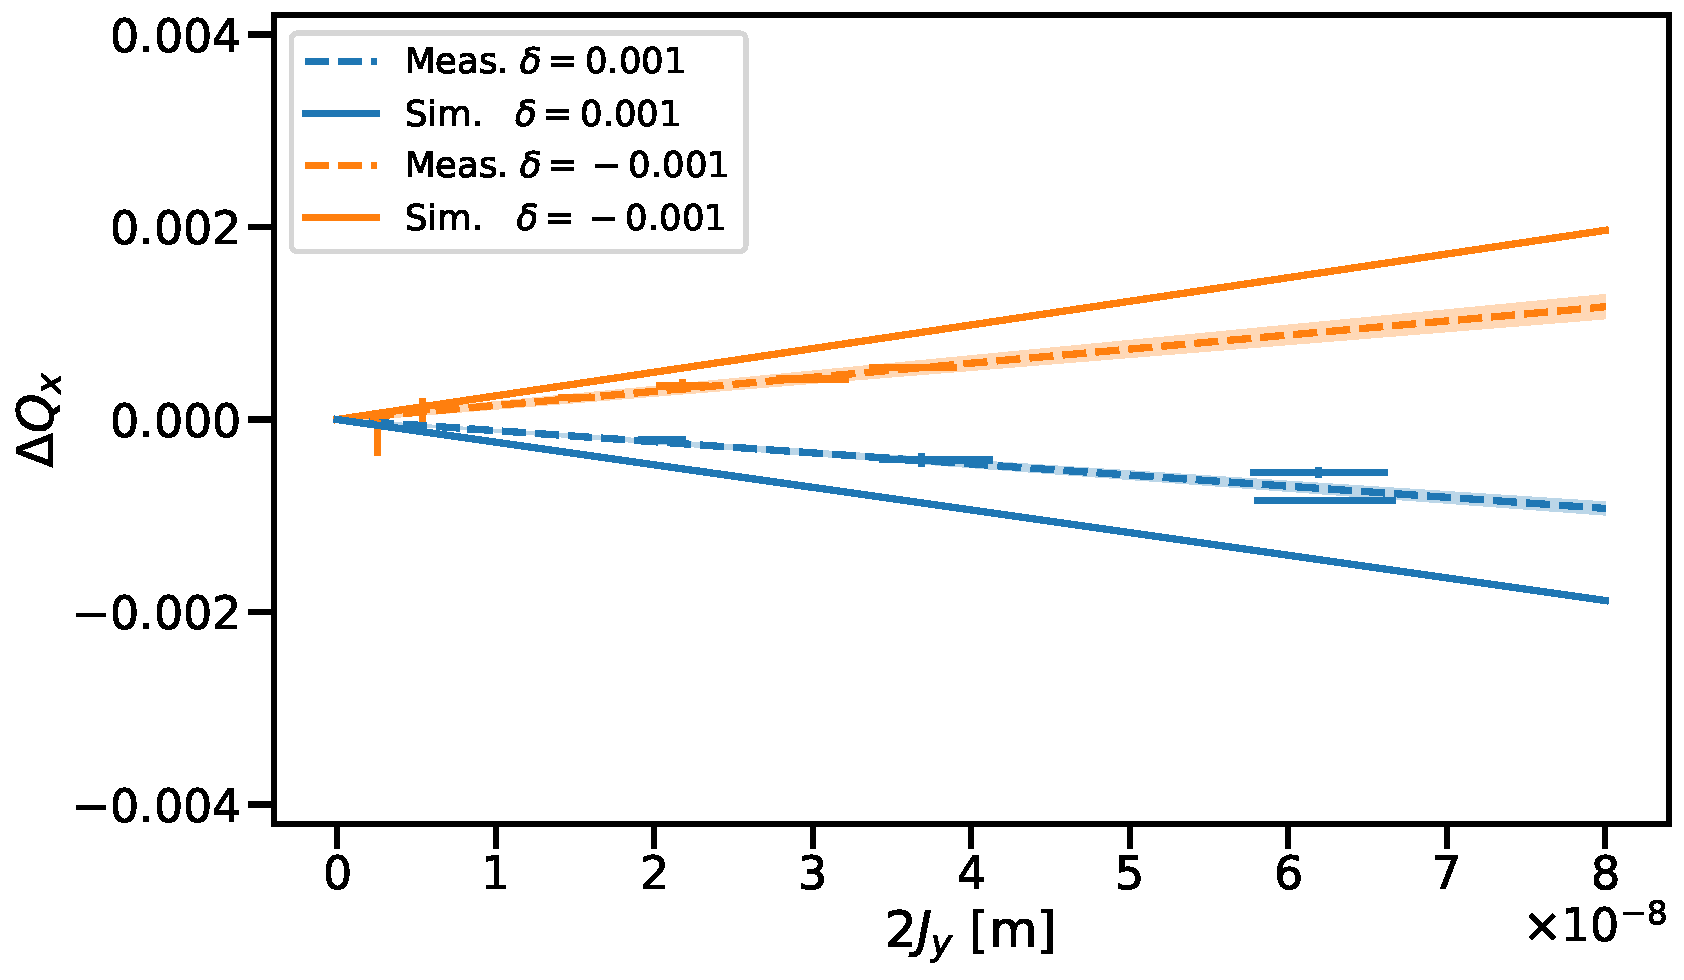
\includegraphics[width=\textwidth]{images/chromatic_amplitude_detuning/B2_Qxy_decay0.47.pdf}
      \caption{Horizontal tune shift depending on the vertical action: 
      $\frac{\partial^2 Q_x}{\partial J_y \partial \delta}$.}
      \label{figure:decapoles:decay:b2qxy}
  \end{subfigure}
  %
  \\[1em]
  %
  \begin{subfigure}{0.8\textwidth}
      \centering
      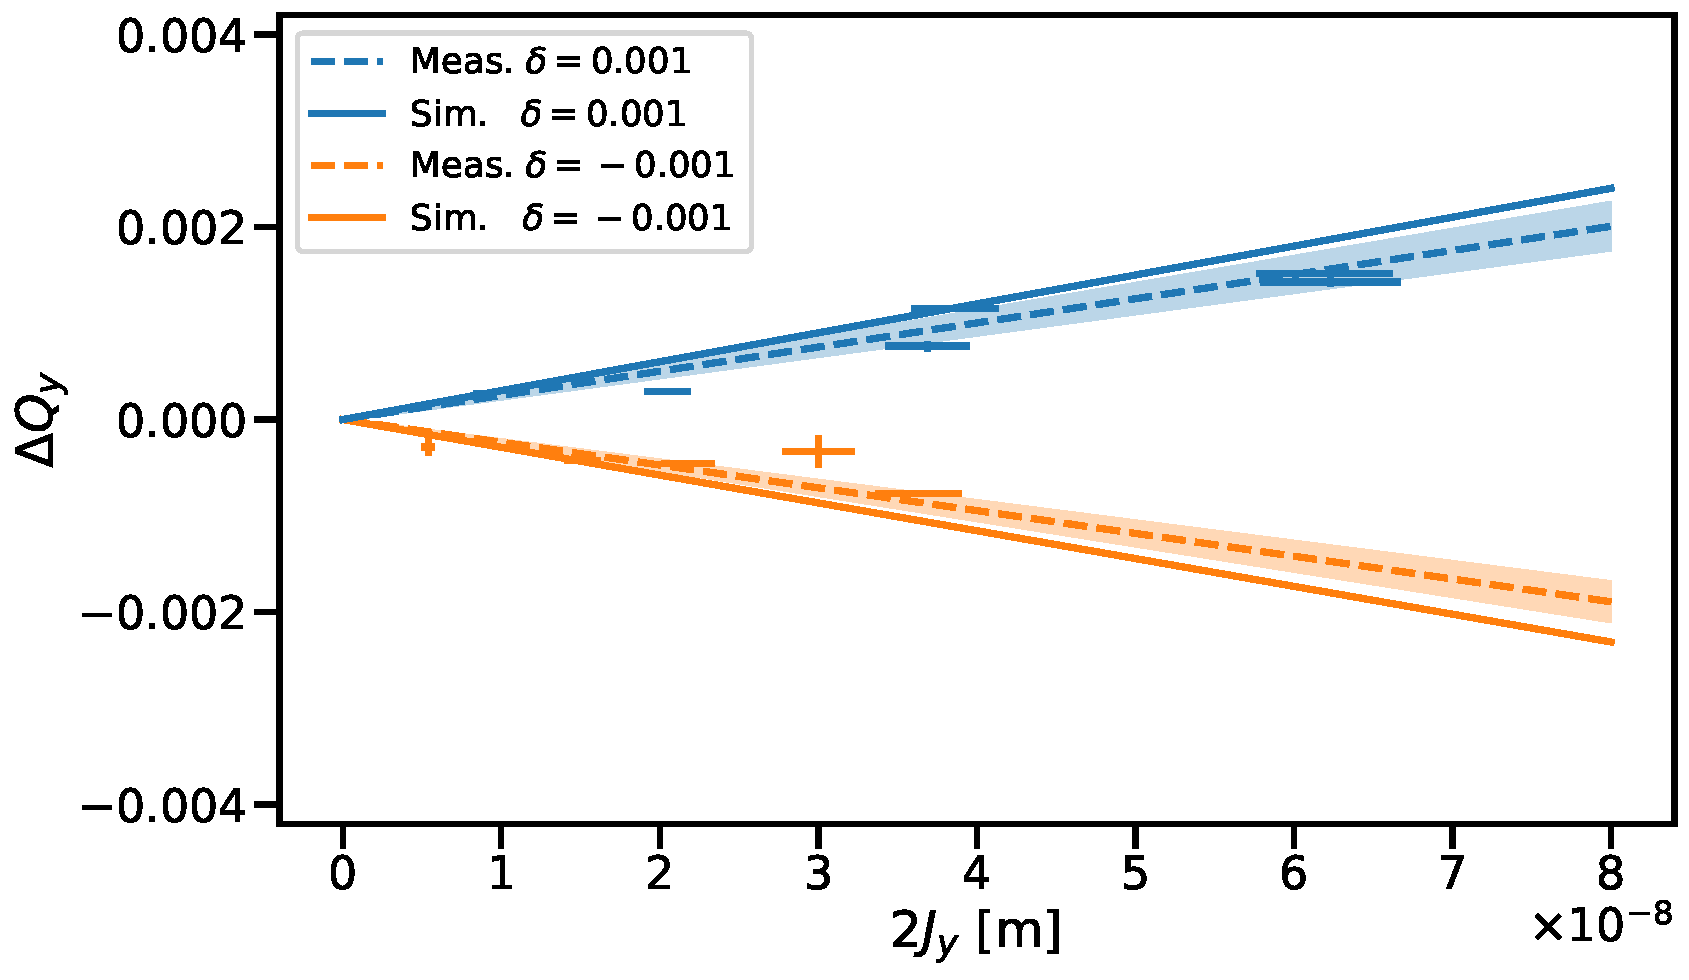
\includegraphics[width=\textwidth]{images/chromatic_amplitude_detuning/B2_Qyy_decay0.47.pdf}
      \caption{Vertical tune shift depending on the vertical action: 
      $\frac{\partial^2 Q_y}{\partial J_y \partial \delta}$.}
      \label{figure:decapoles:decay:b2qyy}
  \end{subfigure}
  \caption{Measured and simulated tune shift depending on the action at two different momentum
  offsets. Each fit corresponds to a chromatic amplitude detuning term evaluated at a certain
  $\delta$. Estimates from simulations are lowered due to the $b_5$ decay of the main dipoles.}
  \label{figure:decapoles:decay:two_terms}
\end{figure}

